\documentclass[a4paper,12pt]{report}

\usepackage{cmap}
\usepackage[T2A]{fontenc}
\usepackage[utf8]{inputenc}
\usepackage[russian]{babel}
\usepackage{amsmath,amsfonts,amssymb}
\usepackage{graphicx}
\usepackage{sidecap}
\usepackage{wrapfig}
\usepackage{indentfirst}

\begin{document} 

\begin{titlepage} 

\begin{center} 

\large Федеральное государственное автономное образовательное учреждение высшего образования «Санкт-Петербургский государственный электротехнический университет «ЛЭТИ» им. В.И. Ульянова (Ленина)»\\
кафедра Вычислительной техники\\[5cm] 

\huge ОТЧЕТ\\ по лабораторной работе № 8\\[0.5cm] 
\large <<Линейные односвязные списки>>\\[3.7cm]

\begin{minipage}{1\textwidth}
    \begin{flushleft}
        \emph{Автор:} Стукен В.А.\\
        \emph{Группа:} 2307\\
        \emph{Факультет:} ФКТИ\\
        \emph{Преподаватель:} Аббас Саддам Ахмед\\
    \end{flushleft}
\end{minipage}

\vfill

Санкт-Петербург, 2023\\
{\large \LaTeX}

\end{center}
\thispagestyle{empty}
\end{titlepage}

\section*{Задание(вариант 13)}
Разработать подалгоритм, обеспечивающий копирование элемента списка с заданным id в заданную позицию 
(0 считается позицией «перед первым элементом») с одновременным автоинкрементом поля id. 
Если номер позиции превышает количество элементов списка, копирование делается в позицию «после последнего».
\section*{Постановка задачи и описание решения}
\par

Сначала создаем голову односвязного списка(ф-ция make-head()) Затем просим ввести id элемента, и позицию куда будем вставлять элемент.
Далее открываем файл, создаем в цикле новый Node и заполняем его данными и присваиваем id. Потом находим по введенному пользователем id ищем Node с таким id(ф-ция search-by-id()) и копируем этот элемент на введенную пользователем позицию(ф-ция insert-after())
В самом конце выводим полученный список(ф-ция print())


\section*{Описание переменных-функция main}
\begin{centering}
\resizebox{14cm}{!}{
    \begin{tabular}{|l|l|l|l|}
        \hline
        \textbf{№} & \textbf{Имя переменной} & \textbf{Тип} & \textbf{Назначение}\\
        \hline
        1 & fp         &FILE*& Указатель на файл\\ 
        \hline
        2 &  S,S0           & Node*  & Указатели на узлы списка\\ 
        \hline
        3 &  H   &  Head* & Указатель на голову списка \\
        \hline
        4 & s1        & char[] & Строка файла\\ 
        \hline
        5 & s2           & char[][] & Двумерный массив строк \\
        \hline
        6 & slen    & int & Длина строки \\
        \hline
        7 & number    & int & Id элемента \\
        \hline
        8 & position   & int & Позиция, куда надо скопировать эл. \\
        \hline
        9 & target-node   & Node* & Указатель на элемент с указанным id\\
        \hline
        10 & node-after & Node* & Указатель на элемент на определенной позиции \\
        \hline
    \end{tabular}
}
\end{centering}
\section*{Примеры работы программы:}
\begin{figure}[ph]
    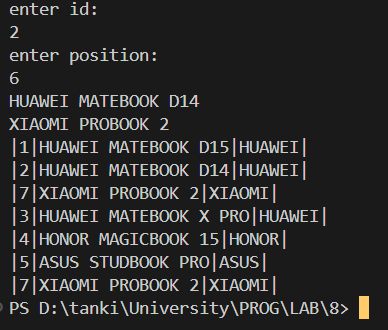
\includegraphics[width=0.6\textwidth]{ex1.jpg}
\caption{Пример 1}
\label{ris:image1}
    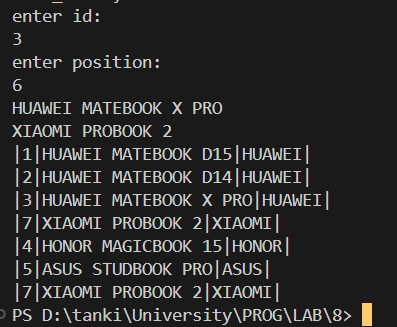
\includegraphics[width=0.7\textwidth]{ex2.jpg}
\caption{Пример 2}
\label{ris:image2}
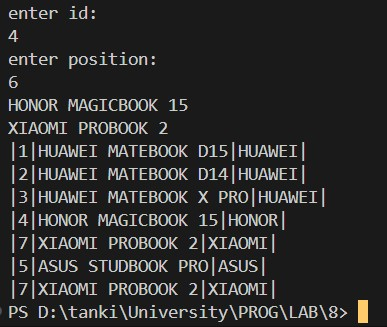
\includegraphics[width=0.7\textwidth]{ex3.jpg}
\caption{Пример 3}
\label{ris:image3}

\end{figure}


\newpage

\section*{Вывод}
В данной лабораторной работе научились работать с односвязными списками в языке Си, 
реализовали простейший алгоритм копирования элемента односвязного списка на определенную позицию.
\end{document}